\documentclass{beamer}
\usetheme{Warsaw}
\usepackage{nhtvslides}
\usepackage{graphicx}
\usepackage{amssymb}
\usepackage{pifont}
\usepackage{listings}
\lstset{language=CAML,
basicstyle=\ttfamily\footnotesize,
frame=shadowbox,
breaklines=true}
\usepackage[utf8]{inputenc}

\newcommand{\cmark}{\ding{51}}%
\newcommand{\xmark}{\ding{55}}%

\title{Casanova 2.0}
\subtitle{A basic introduction}

\author{Dr. Giuseppe Maggiore}

\institute{NHTV University of Applied Sciences \\ 
Breda, Netherlands}

\date{}

\begin{document}
\maketitle

\section{About games}
\begin{slide}{Game development}{Interests}{
\item A huge field
\item Increasing artistic and narrative value \cite{GAMES_ART_NARRATIVE}
\item Largely unexplored potential fields of application
}\end{slide}

\begin{frame}{Games sales}
\center
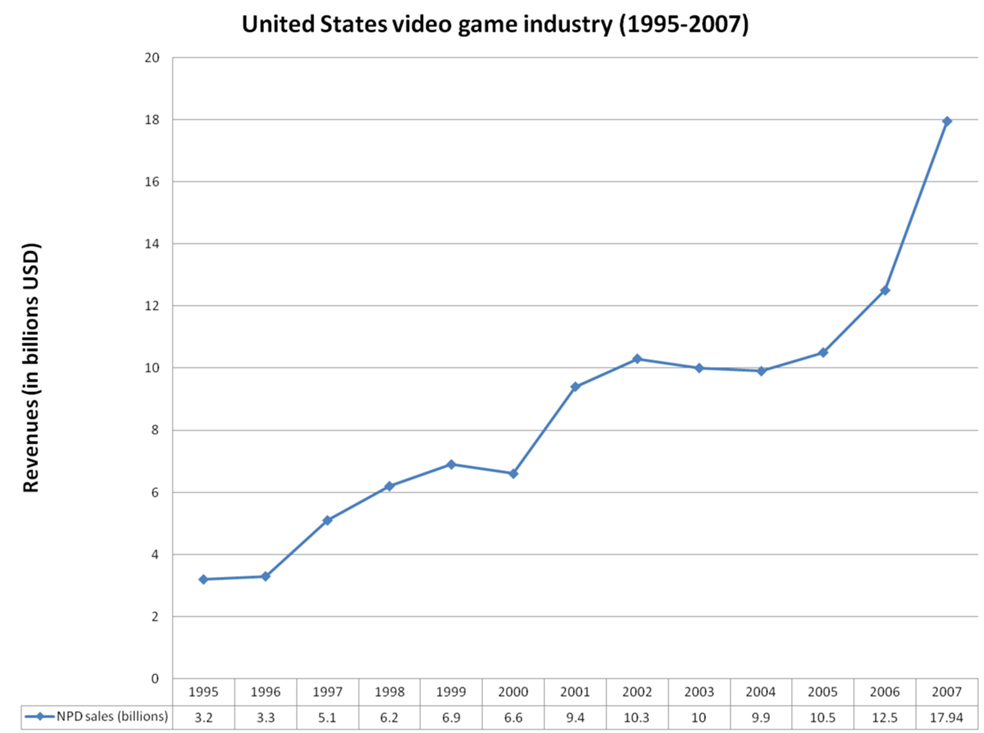
\includegraphics[height=5cm]{Pics/games_sales.png}
\end{frame}

\begin{slide}{Game development}{Fields of application}{
\item As a supporting tool for training \cite{GAMES_FOR_TRAINING}
\begin{itemize}
\item \textit{military}
\item \textit{crane operation}
\item \textit{medicine}
\item ...
\end{itemize}
}\end{slide}

\begin{frame}{Games for training}
\center
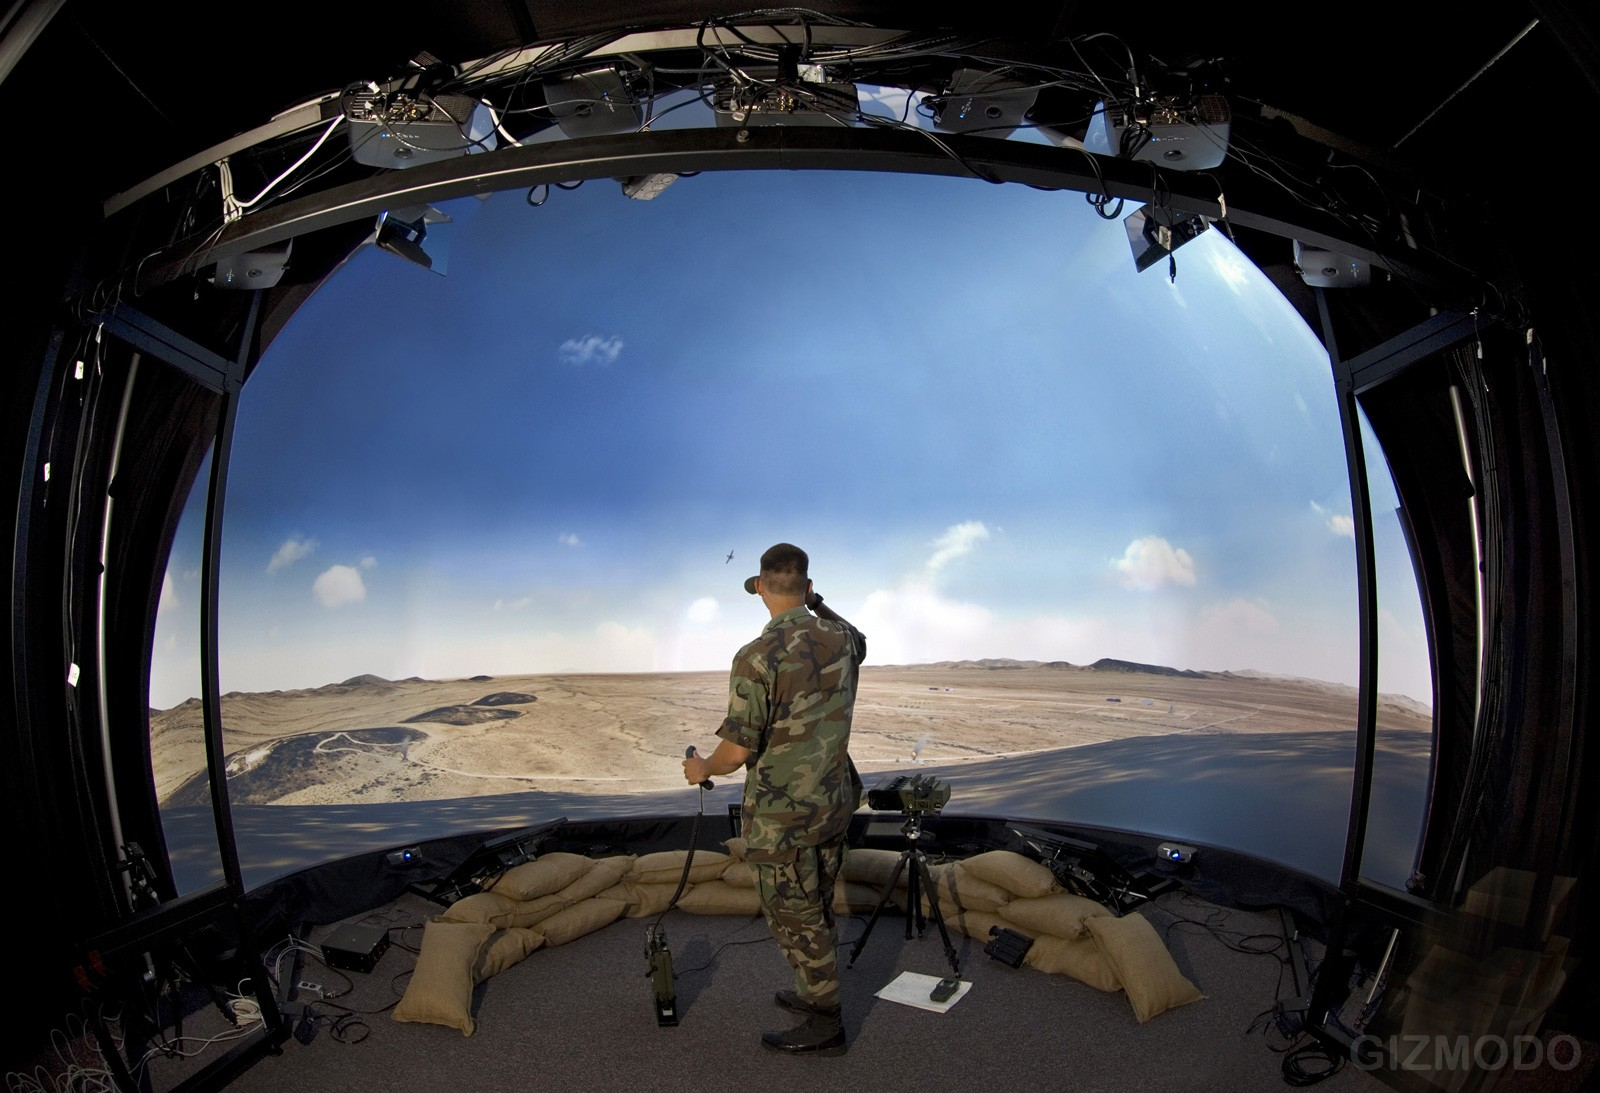
\includegraphics[height=5cm]{Pics/military_simulator.png}
\end{frame}

\begin{frame}{Games for training}
\center
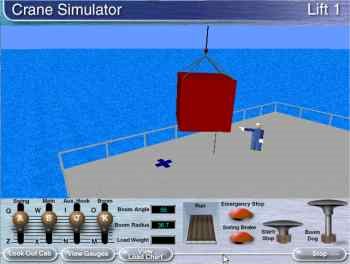
\includegraphics[height=5cm]{Pics/crane_simulator.png}
\end{frame}

\begin{frame}{Games for training}
\center
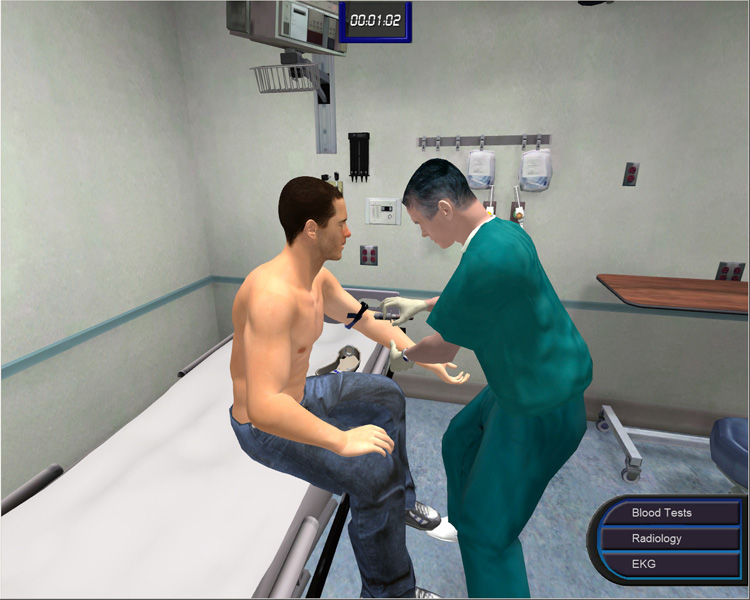
\includegraphics[height=5cm]{Pics/medical_simulator.png}
\end{frame}

\begin{slide}{Game development}{Fields of application}{
\item As a supporting tool for education \cite{GAMES_FOR_EDUCATION}
\begin{itemize}
\item Math
\item Chemistry
\item History
\item ...
\end{itemize}
}\end{slide}

\begin{frame}{Games for education}
\center
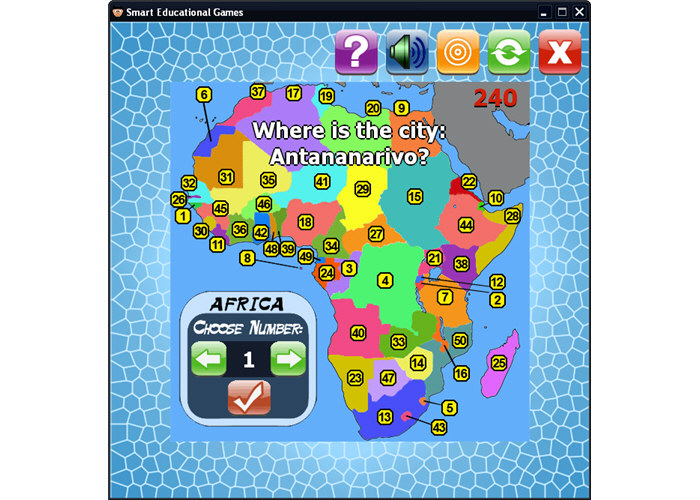
\includegraphics[height=5cm]{Pics/game_for_education.png}
\end{frame}

\begin{slide}{Game development}{Fields of application}{
\item As a supporting tool for research
\begin{itemize}
\item Psychology \cite{GAMES_FOR_LANGUAGE_LEARNING}
\item Philosophy
\item AI \cite{GAMES_FOR_AI_RESEARCH}
\item ...
\end{itemize}
}\end{slide}

\begin{frame}{Games for research}
\center
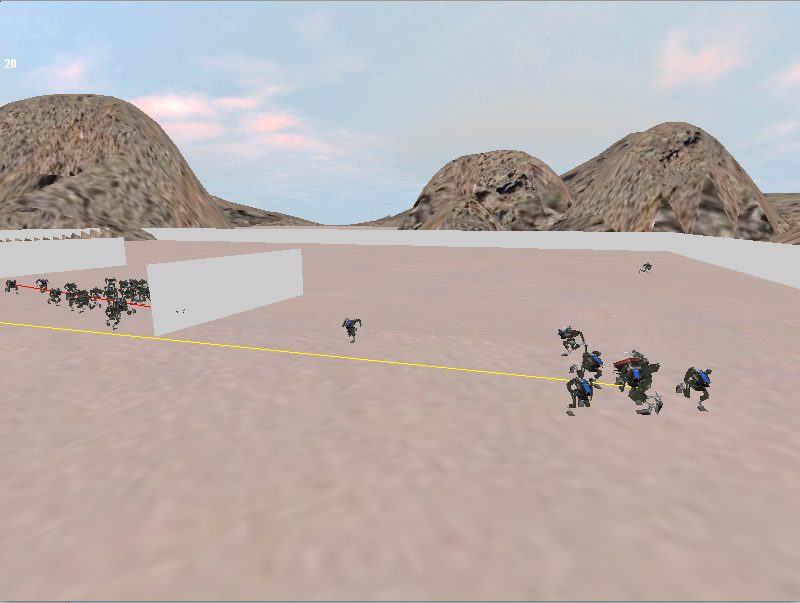
\includegraphics[height=5cm]{Pics/game_for_ai.png}
\end{frame}

\begin{frame}{Games for research}
\center
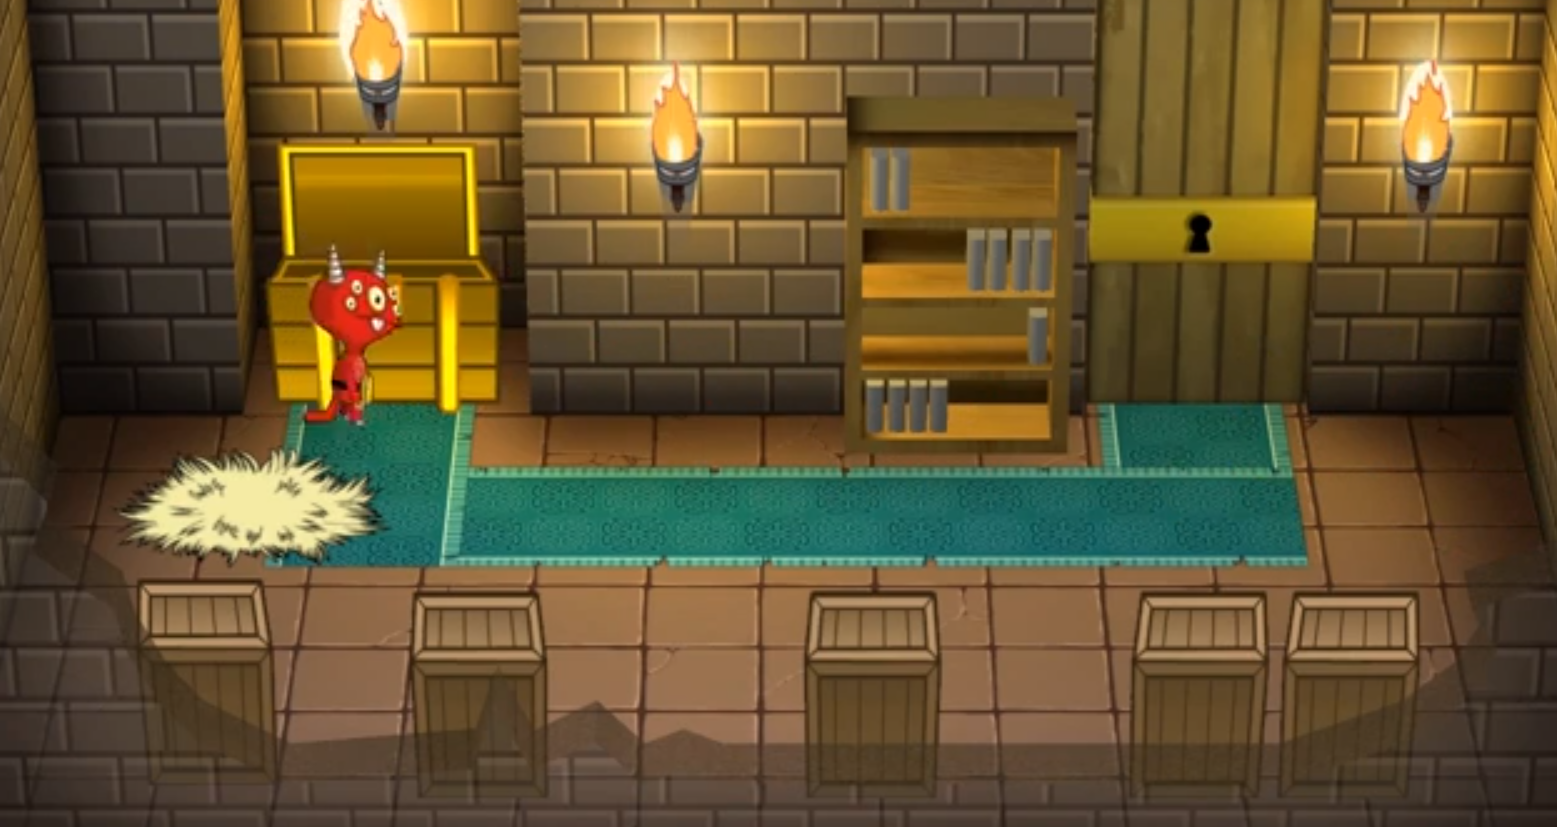
\includegraphics[height=5cm]{Pics/game_for_philosophy.png}
\end{frame}

\begin{frame}{Games for research}
\center
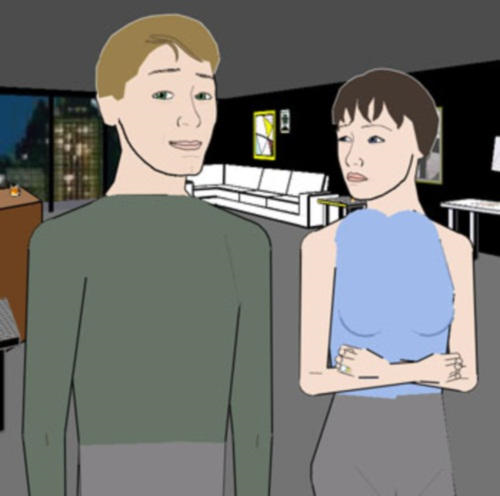
\includegraphics[height=5cm]{Pics/game_for_psichology.png}
\end{frame}

\begin{slide}{Game development}{Unexplored?}{
\item So many opportunities: \textbf{why is it unexplored?}
\pause
\item Because it is incredibly expensive to make an even decent game \item Low-quality game means distraction because of poor interaction
}\end{slide}

\begin{frame}{Games for research}
\center
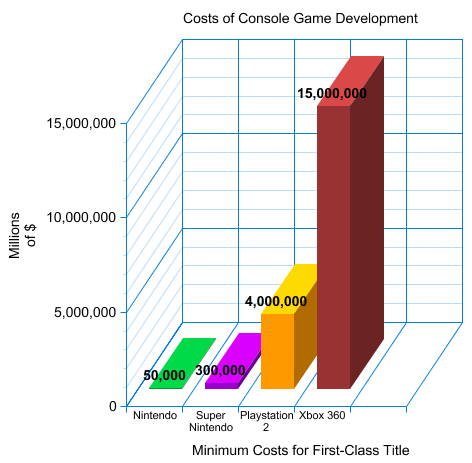
\includegraphics[height=5cm]{Pics/game_development_costs.png}
\end{frame}

\begin{slide}{Game development}{Why is it expensive?}{
\item Art is expensive
\begin{itemize}
\item Procedural generation \cite{PROCEDURAL_GENERATION} moves some cost from art to programming
\end{itemize}
\item Programming is expensive
\begin{itemize}
\item Most programming technology is \textit{inadequate} for games
\item It is designed for other fields of application
\item Lots of time for trivial tasks
\item Lots of time for debugging
\end{itemize}
}\end{slide}

\begin{slide}{Game development}{Taming the costs}{
\item Reuse code and art
\item Can yield games similar to each other (surprise there!)
}\end{slide}

\begin{slide}{Game development}{Reusing code and art}{
\item Does not help us at all!
\item Research and education games are inherently different
\item We need \textit{cheap} and \textit{fast} ways to prototype
}\end{slide}

\section{Casanova language}
\begin{slide}{Casanova language}{Basics}{
\item Build a programming language \textit{exclusively for making games}
\item Syntax and semantics are focused on the primitives of simulation
\begin{itemize}
\item \cmark \textit{Transformation} of the game world as time progresses
\item \cmark \textit{Time} as a first class primitive
\item \cmark \textit{Parallel update} of many things at once
\item \cmark Collection-oriented programming
\item \cmark Math-oriented programming
\item \cmark Pluggable game engines
\item \cmark Saving and loading
\end{itemize}
}\end{slide}

\begin{slide}{Casanova language}{Basics}{
\item Build a programming language \textit{exclusively for making games}
\item Syntax and semantics are focused on the primitives of simulation
\begin{itemize}
\item \xmark IDE integration
\item \xmark Lots of samples (for our own debugging)
\item \xmark Networking primitives
\item \xmark Object-orientation
\item \xmark SQL-style optimization
\item \xmark Static/dynamic analysis framework to detect errors
\item \xmark Graphics-oriented language subset (CNSL)
\end{itemize}
}\end{slide}

\begin{slide}{Casanova language}{Basic semantics}{
\item \textbf{Rules}: a series of transformations of the world
\item Each repeated with a variable time step ($\delta t_{ij} \leq \delta t_{\text{min}}$)
\item Merged together automatically

\begin{align*}
r_1 &: w_{10} \underbrace{\rightarrow}_{\delta t_{11}} w_{11} \underbrace{\rightarrow}_{\delta t_{12}} w_{12} \underbrace{\rightarrow}_{\delta t_{13}} \dots \underbrace{\rightarrow}_{\delta t_{1n}} w_{1n} \\
r_2 &: w_{20} \underbrace{\rightarrow}_{\delta t_{21}} w_{21} \underbrace{\rightarrow}_{\delta t_{22}} w_{22} \underbrace{\rightarrow}_{\delta t_{23}} \dots \underbrace{\rightarrow}_{\delta t_{2n}} w_{2n} \\
\vdots \\
r_m &: w_{m0} \underbrace{\rightarrow}_{\delta t_{m1}} w_{m1} \underbrace{\rightarrow}_{\delta t_{m2}} w_{m2} \underbrace{\rightarrow}_{\delta t_{m3}} \dots \underbrace{\rightarrow}_{\delta t_{mn}} w_{mn}
\end{align*}
}\end{slide}

\begin{frame}[fragile]{Sample 1 - hello world}
\begin{lstlisting}
world HelloWorld = {
  Text  : Text
}

let world = {
  Text = Text.Create("Hello Casanova!", 
           Vector2<pixel>(0.0f, 0.0f), 
           Vector2<pixel>(200.0f, 200.0f))
}
\end{lstlisting}
\end{frame}

\begin{frame}[fragile]{Sample 2 - animation}
\begin{lstlisting}
world SimpleAnimation = {
  Text        : Text
  Position    : Vector2<pixel>
  Velocity    : Vector2<pixel/s>
  Checkpoints : List<Vector2<pixel>>
} with
  rule Position = self.Position + self.Velocity * dt
  rule Velocity = 
    for c in self.Checkpoints do
      yield Vector2.Normalize(c - self.Position) * 10.0f<pixel/s>
      wait_until (Vector2.Distance(c, self.Position) <= 0.1f<pixel>)
\end{lstlisting}
\end{frame}


\section{Dyslexia detection in young children}
\begin{slide}{Case study}{A game for dyslexia detection in children}{
\item Pairs of sounds; say if equal or different
\item Children get bored really quickly
}\end{slide}


\begin{frame}{That's it}
\center
\fontsize{18pt}{7.2}\selectfont
Sounds
\end{frame}


\begin{slide}{Case study}{A game for dyslexia detection in children}{
\item Idea: create a frame of ``game mechanics'' around this concept
\item More pleasant environment to perform the tests
\item No visual help or hints
\item Very simple mechanisms
}\end{slide}


\begin{slide}{Case study}{A game for dyslexia detection in children}{
\item Use a tutorial mechanism for initial training (no lengthy explanations)
\item Use lots of animations and visual metaphors to explain the tasks
}\end{slide}


\begin{frame}{Dyslexia game}
\center
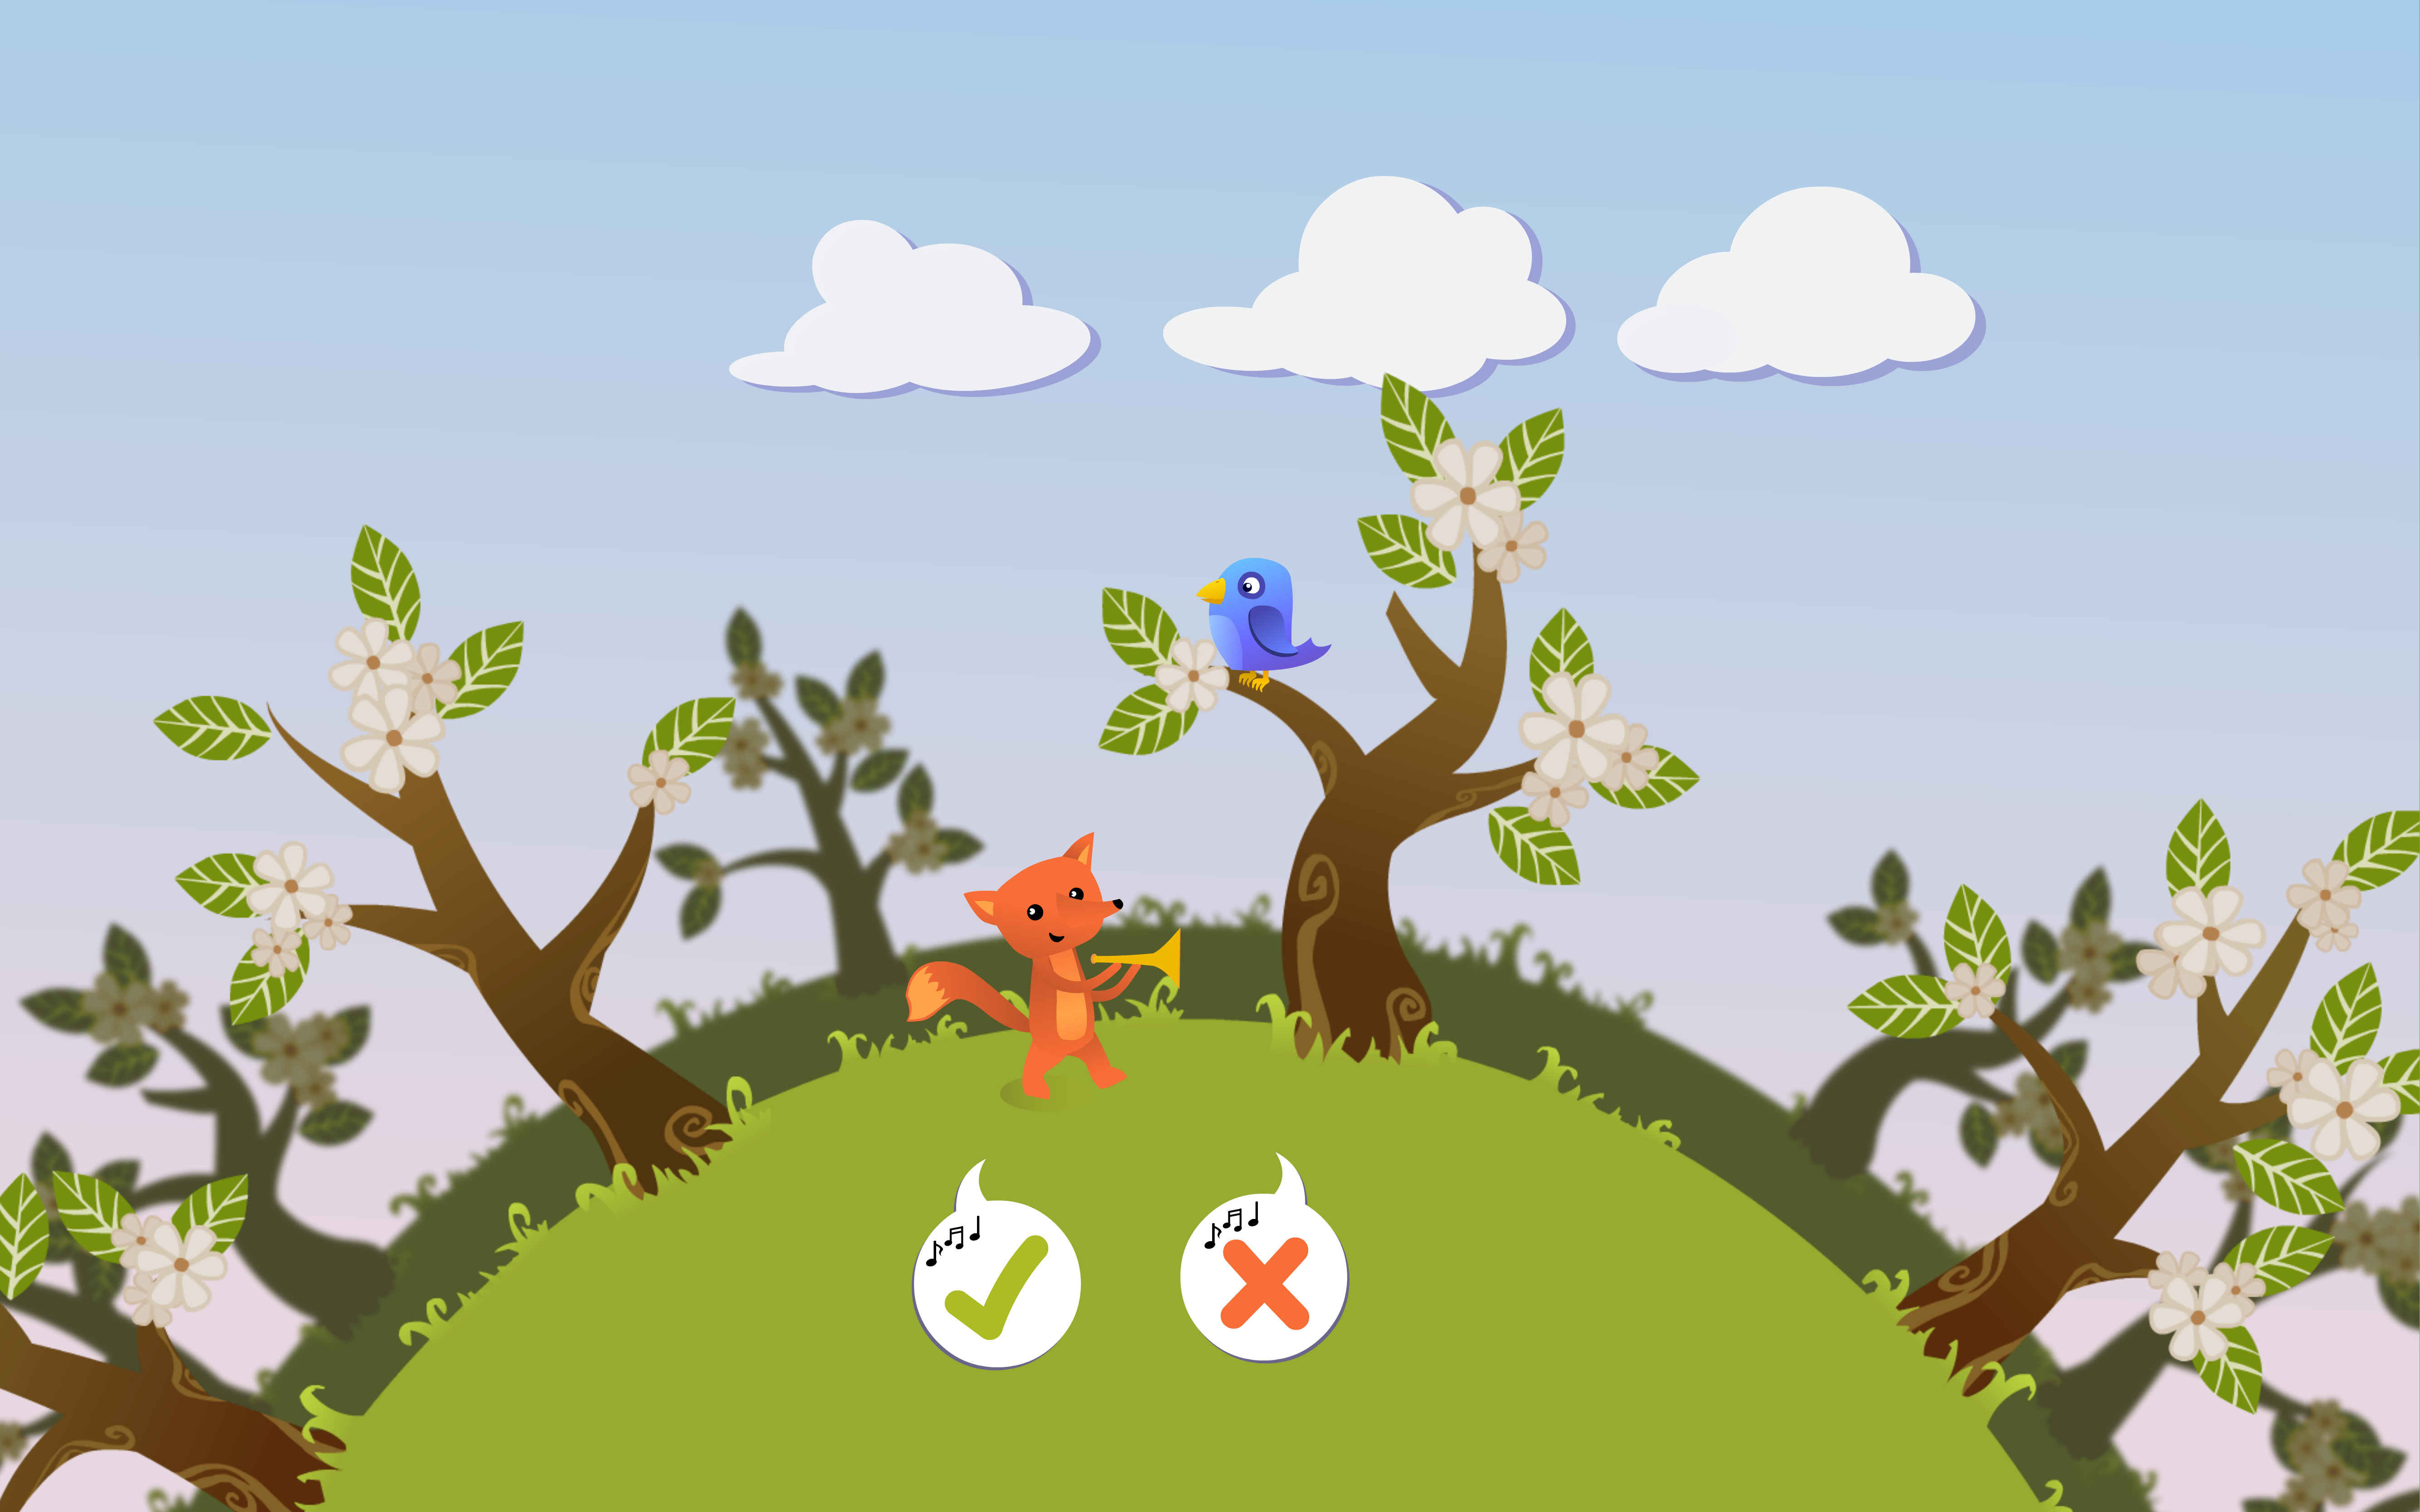
\includegraphics[height=5cm]{Pics/dyslexia_game.png}
\\ Demo!
\end{frame}


\begin{slide}{Case study}{About the implementation}{
\item Huge, nested state machines
\item Lots of prototyping (we built three full versions of the game)
\item Can be done with other tools, but:
\begin{itemize}
\item Casanova helped immensely
\item Our expertise in Casanova contributed a lot
\end{itemize}
}\end{slide}


\begin{frame}{Dyslexia game}
\center
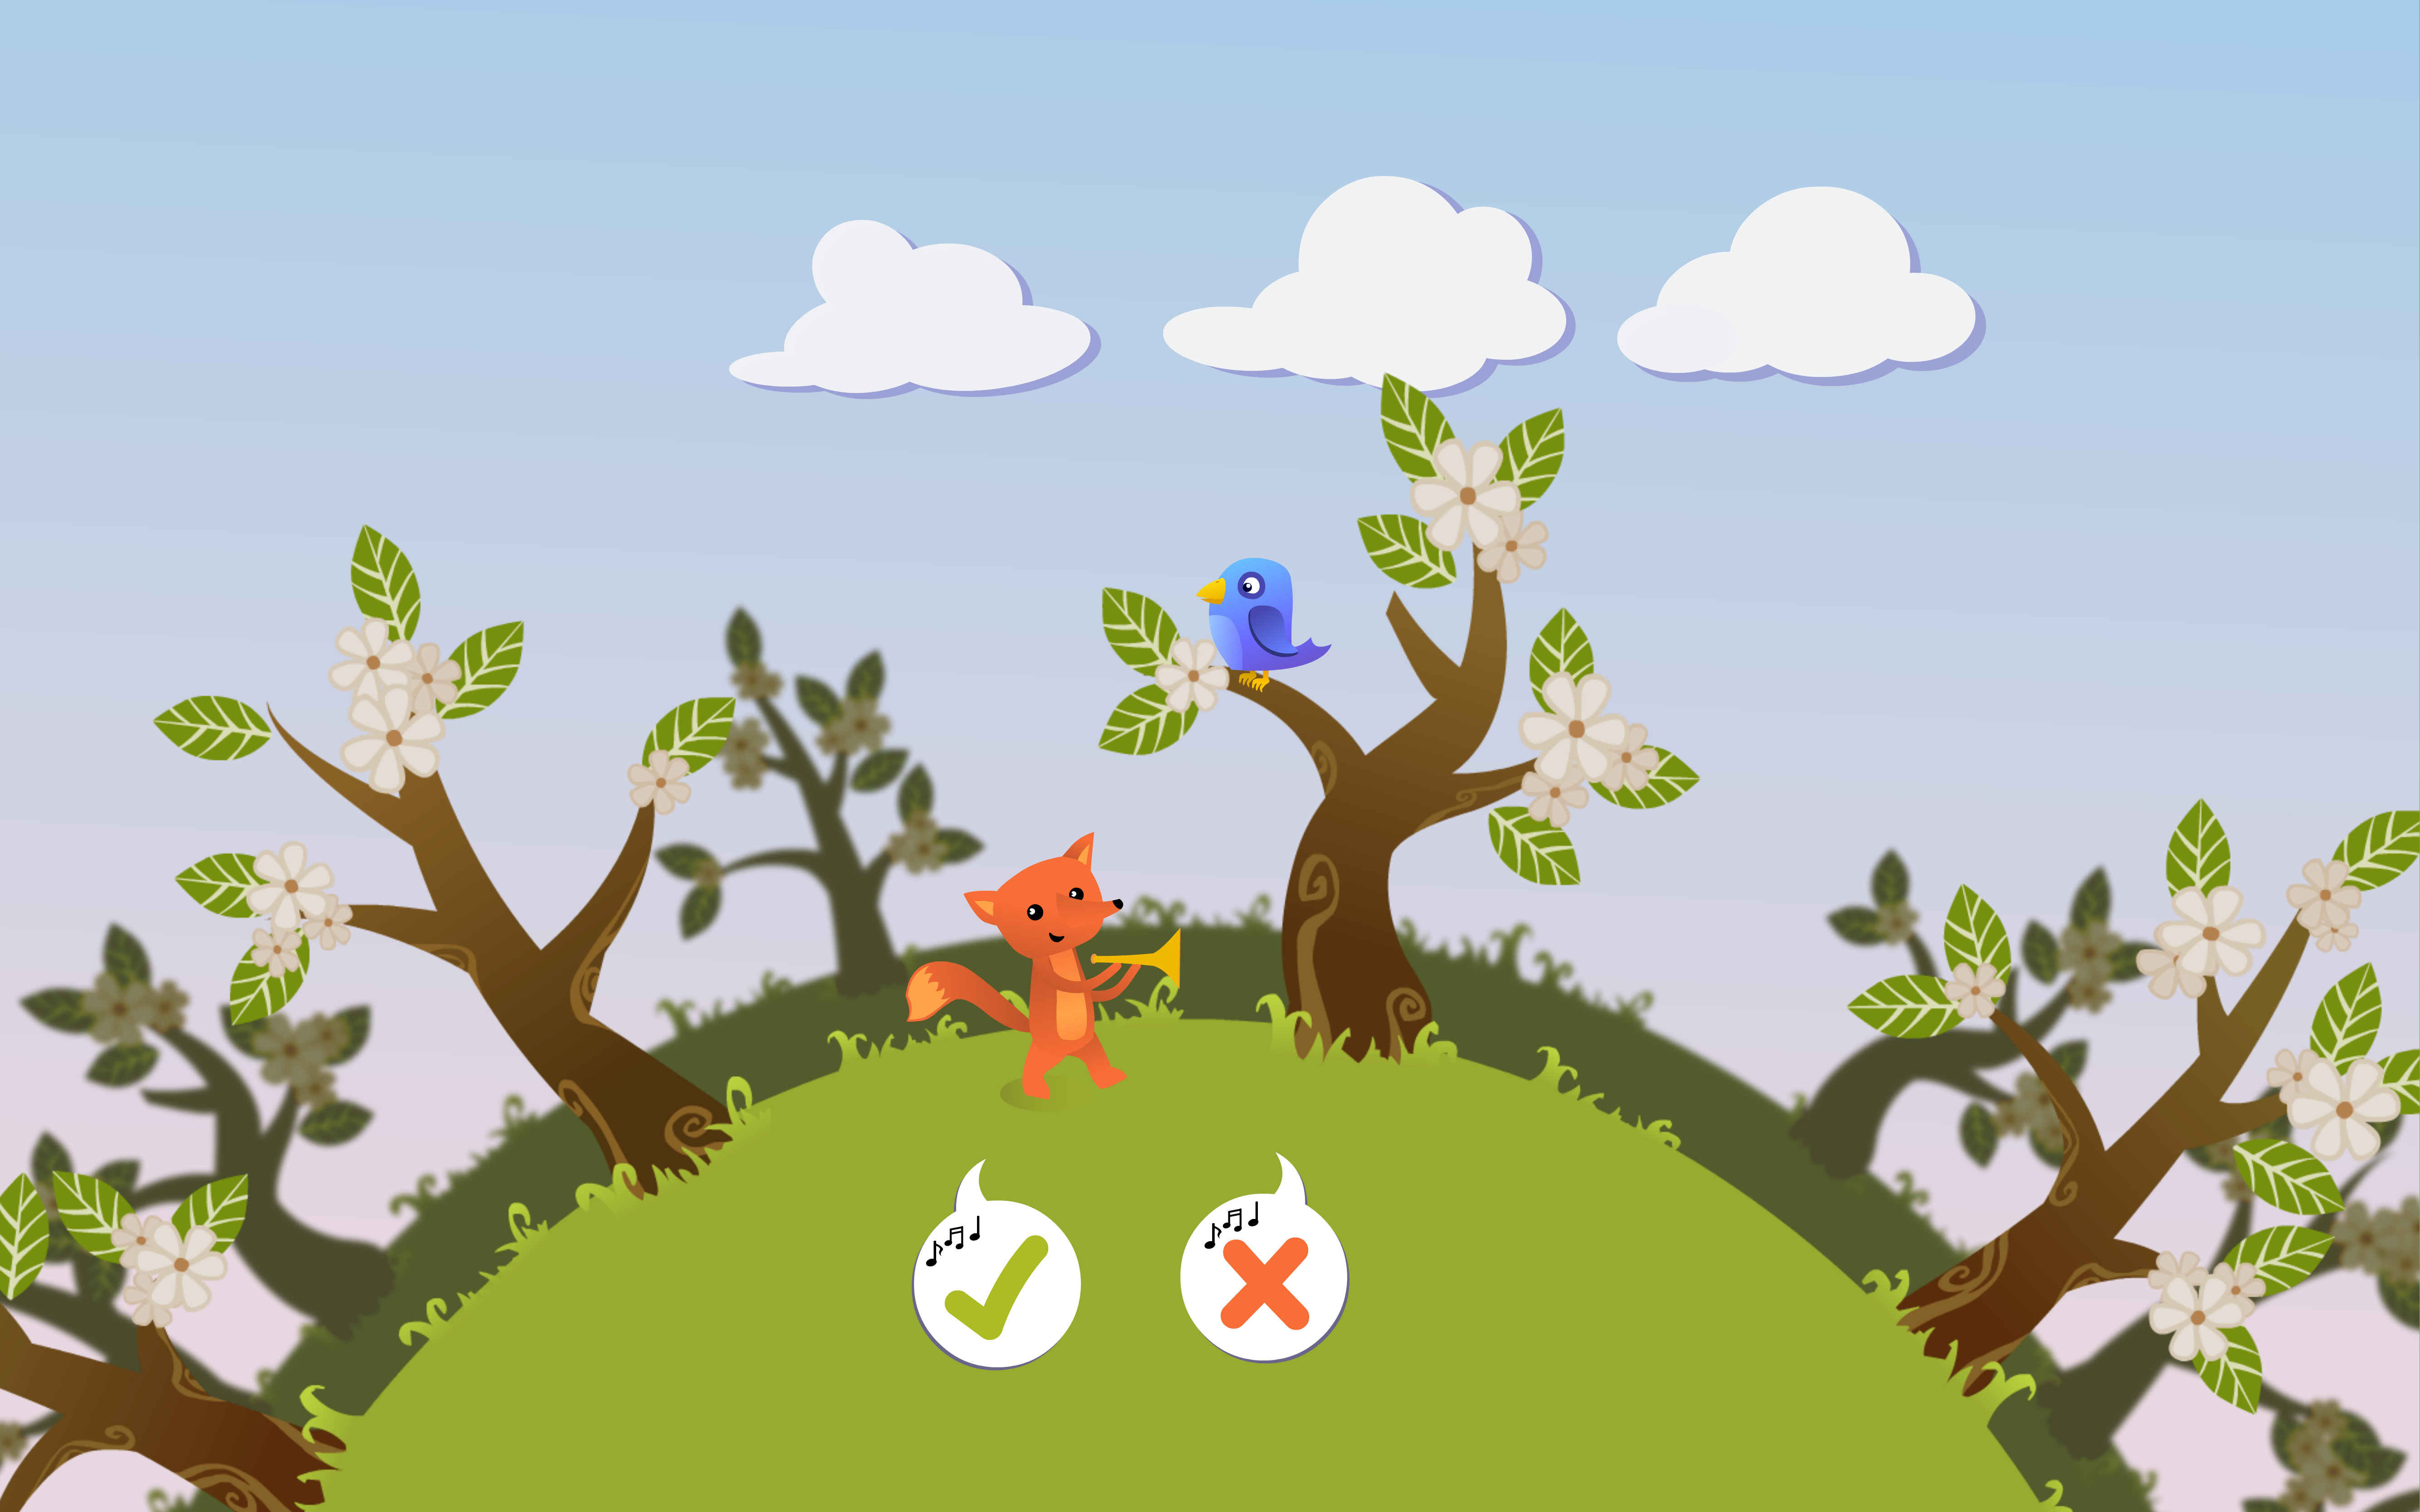
\includegraphics[height=5cm]{Pics/dyslexia_game.png}
\\ Demo!
\end{frame}


\section{Conclusion and future work}
\begin{slide}{Conclusion}{Games and research}{
\item Game development is interesting for research and other novel applications
\item Huge costs make the realization of this infeasible for most practical purposes
\item We propose a novel language built for \textit{fast development} of games
\pause
\item We aim at using this language to speed-up development of research games for third parties
\begin{itemize}
\item We already have a case study
\end{itemize}
\item While building case studies we wish to
\begin{itemize}
\item Perfect the quality of our technology
\item Add ``killer features'' like networking for bigger customers
\end{itemize}
}\end{slide}


\begin{frame}{That's it}
\center
\fontsize{18pt}{7.2}\selectfont
Thank you!
\end{frame}

\begin{frame}[allowframebreaks]
\frametitle{References}
\bibliographystyle{plain}
\bibliography{bibliography}
\end{frame}

\end{document}


\begin{slide}{SECTION}{SLIDE}{
\item i
}\end{slide}

\begin{frame}[fragile]{SLIDE}
\begin{lstlisting}
CODE
\end{lstlisting}
\end{frame}

\begin{frame}{SLIDE}
\center
%\includegraphics[height=5cm]{Pics/recursive_multiplier.png}
\end{frame}
